%\documentclass{article}

\section{Zielsetzung}
\label{sec:Zielsetzung}
Ziel des Versuchs ist die Bestimmung des effektiven Saugvermögens der Drehschieberpumpe und der Turbomolekularpumpe
mit Hilfe der Auswertung von Evakuierungskurven und durch Ermittlung ihrer jeweiligen 
Leckraten. Außerdem sollen die Grundlagen der Vakuumphysik, so wie der Umgang mit den entsprechenden Vakuumtechnik-Komponenten
erlernt werden. Die Vakuumphysik hat vielfältige Anwendungsbereiche in Wissenschaft und Industrie. In der Lebensmittelverarbeitung 
wird Vakuumtechnik zum Gefriertrocknen und zur Vakuumverpackung genutzt. In der wissenschaftlichen Forschung ist sie essentiell
für physikalische Experimente und die Massenspektrometrie. Auch im Alltag findet Vakuumtechnik Anwendung, etwa bei der Beschichtung 
von Glas für bessere Isolierung und beim Recycling von Elektroschrott zur Rückgewinnung wertvoller Materialien. Diese vielseitigen 
Einsatzmöglichkeiten machen die Vakuumphysik zu einem unverzichtbaren Werkzeug in vielen Bereichen.

\section{Theorie}
\label{sec:Theorie}

Das Vakuum ist ein Zustand geringer Gasdichte, also ein Raum, welcher Nahezu leer von Materie ist.
Da dieser Raum nur wenige Teilchen enthält, ist der Druck in einem Vakuum deutlich geringer als der Atmosphärendruck.
Druck ist definiert als die Kraft pro Fläche, die von Gasmolekülen ausgeübt wird, wenn sie auf
eine Oberfläche stoßen. Die mittlere freie Weglänge, also die Strecke, welche ein Teilchen im Mittel zurücklegt, bevor es
mit einem anderen kollidiert, ist folglich sehr hoch. Ein perfektes Vakuum ist in der Praxis nicht zu realisieren, zur mathematischen 
beschreibung des Vakuums wird die Zustandsgleichungen des idealen Gases verwendet, einem theoretischen Modell für ein 
Gas, in welchem die Teilchen keine Wechselwirkungen außer elastischen Stößen erfahren. Außerdem ist ihr Volumen vernachlässigbar 
und sie werden als Punktförmige Teilchen angenommen.
Die Zustandsgleichung des idealen Gases ist gegeben durch
\begin{equation}
     p V=N k_\text{B} T .
    \label{eq:idealgaslaw}
\end{equation}  
Dabei ist \( p \) der Druck, \( V \) das Volumen, \( N \) die Teilchenanzahl, \( k_B \) die Boltzmann-Konstante
 und \( T \) die Temperatur.
Bei konstanter Temperatur ist der Druck eines Gases umgekehrt proportional zum Volumen, das ist das Boyle-Mariottesche Gesetz,
\begin{equation}
    \frac{p_1}{p_2}=  \frac{V_2}{V_1}.
    \label{eq:boylemariotte}
\end{equation}


\subsection{Druckbereiche und Strömungsarten}


Beim Evakuierungsvorgang fällt der Druck über die Zeit. Der normale Atmosphärendruck beträgt auf der Erdoberfläche 1 bar.
Die Druckbereiche des Vakuums liegen bei folgenden Werten:
Grobvakuum bei 1 bar bis $10^{-3}$ bar,  Feinvakuum von $10^{-3}$ bar bis $10^{-7}$ bar, Hochvakuum von $10^{-7}$ bis $10^{-9}$ bar und
das Ultrahochvakuum liegt bei Werten unter $10^{-9}$ bar.
In niedrigen Druckbereichen, also im Hochvakuum und im Ultrahochvakuum, dominiert die molekulare Strömung, hier bewegen sich die Moleküle fast unabhängig voneinander,
da sie nur selten kollidieren und ihre mittlere freie Weglänge größer ist als die Abmessunge des Behälters.
In größeren Druckbereichen kollidieren die Teilchen oft 
und bewegen sich in geordneten Bahnen, das wird laminare Strömug genannt.
Im folgenden betrachten wir ein Gemisch aus Gasen, der Gesamtdruck ist dabei die Summe aller Partialdrücke. Der Partialdruck eines Gases in
einem Gasgemisch ist der Druck, den dieses einzelne Gas ausüben würde, wenn es alleine das gesamte Volumen des Gemisches ausfüllen würde.

\subsection{Partialdrücke der Luft}
Der Versuch wird mit Luft betrieben, die präzise Zusammensetzung dieser und der Partialdrücke ist von äußerster Wichtigkeit.
Luft besteht hauptsächlich aus Stickstoff, Sauerstoff, Argon und Kohlendioxid, zusammen mit geringen Mengen anderer Gase. 
Hier sind die ungefähren Anteile und die entsprechenden Partialdrücke bei einem Gesamtdruck von 1 atm (101325 Pa):

\begin{align*}
\text{Stickstoff} (N_2) &= 78\% \\
\text{Sauerstoff} (O_2) &= 21\% \\
\text{Argon} (Ar) &= 0.93\% \\
\text{Kohlendioxid} (CO_2) &=0.04\% \\
\text{Andere Gase} &=0.03\% 
\end{align*}


\subsection{Oberflächenphänomene und Gasdynamik}


Um das Verhalten von Gasen in Vakuumexperimenten zu verstehen, müssen sich einige Phänomene klargemacht werden.
Die Moleküle haben alle
eine kinetische Energie, dadurch können sie im Vakuum von einem Bereich hoher Konzentration zu einem Bereich niedriger Konzentration 
gelangen. Diese so genannte Diffusion gewährleistet die Homogenität des Vakuums, kann aber durch Temperaturveränderung und Materialeigenschaften
beeinflusst werden. Haften Gas oder Flüssigkeitsmoleküle an der Oberfläche eines Feststoffes, dringen aber nicht in ihn ein, so wird 
von Adsorption gesprochen. Die Ursache von Adsorption sind oft Van-der-Waals-Kräfte, die zur beschriebenen Anreicherung von Gasen nahe der Oberfläche führen.
Dringen die Moleküle tatsächlich in den Feststoff ein, so handelt es sich um Absorption. Die Moleküle können dort chemisch gebunden oder 
gelöst werden. Im Vakuum tritt Absorption seltener auf als Adsorption. Beide Phänomene können zu einer Druckänderung des Systems führen,
da die Prozesse reversibel sind, die Moleküle können also wieder freigesetzt werden. Dieser Prozess werden als Desorption bezeichnet und kann z.B. durch erhitzen
 erreicht werden. Die Reversibilität der ersten Prozesse ist wichtig für die Aufrechterhaltung eines stabilen Vakuums, führt aber automatisch zu einem Druckanstieg. 
Werden Gase langsam aus Materialien freigesetzt, entstehen virtuelle Lecks im Vakuum. Ihr Ursprung liegt immer in interner Gasfreisetzung, 
sie entstehen nicht durch externe Quellen oder Leckagen.
Leckagen bezeichnen das ungewollte Eindringen von Gas oder Flüssigkeiten durch undichte Stellen in einem System. In der Vakuumtechnik und Physik bezieht sich der Begriff
speziell auf das Eindringen von Luft oder anderen Gasen in ein Vakuumsystem. Leckagen können durch verschiedene Ursachen entstehen wie z.B.
kleine Löcher in den Materialien, beschädigte Dichtungen oder undichte Koppelstellen.
Treten virtuelle Lecks auf, so können sie den Evakuierungsvorgang verlangsamen.

\subsection{Leistung und Effizienz von Vakuumpumpen}


Die Kenngrößen einer Vakuumpumpe sind wichtig um ihre Effizienz und ihre Arbeitsweise zu analysieren.
Der Gasstrom in einer Pumpe beschreibt die Menge an Gas, die pro Zeiteinheit durch ein System bewegt wird. Die Saugleistung einer Pumpe ist ihre 
Fähigkeit, Gas aus einem System zu entfernen. Beides wird typischerweise in Liter pro Sekunde angegeben. Die Saugleistung lässt sich berechnen mit

\begin{equation}
    Q=\frac{dpV}{dt}
    \label{eq:saugleistung}
\end{equation}

Dabei ist \( V \) das Volumen und \( t \) die Zeit.
Das Saugvermögen $S$ ist definiert als die maximale Gasmenge, die die Pumpe bei einem bestimmten Druck abpumpen kann. Das Saugvermögen lässt sich 
mit der Evakuierungskurve berechnen und hängt von dem Betriebsdruck ab:
\begin{equation}
    S=\frac{dV}{dt}.
    \label{eq:saugvermögen}
\end{equation} 

In der Praxis treten Leistungsverluste in einer Pumpe auf, Gründe dafür sind thermische Effekte wie Temperaturänderung des Gases,
Viskosität, raue Innenflächen von Rohren und Kollisionsverluste bei hohen Drücken. Es macht daher Sinn, ein effektives Saugvermögen zu definieren.
Es gilt \cite{grundlagen_vakuumtechnik}

\begin{equation}
    \frac{1}{S_{eff}}=\frac{1}{S}+\frac{1}{C}
    \label{eq:effektives_saugvermögen}
\end{equation}   

Der Leitwert \( C \) eines Rohres beschreibt, wie effizient Gas durch das Rohr transportiert wird. Er kann definiert werden über 
den Strömungswiederstand \( R \), welcher beschreibt wie stark der Gasfluss durch das Rohr behindert wird 
und die Druckdifferenz \(\increment p\), die zwischen der Messsonde und der Pumpe herrscht

\begin{equation}
    C=\frac{1}{R}=\frac{Q}{\increment p}
    \label{eq:leitwert1}
\end{equation}

Mit der Formel für den Gasfluss \( Q \) in Abhängigkeit von dem Strömungswiederstand und der Druckdifferenz

\begin{equation}
    Q=\frac{\increment p}{R}
    \label{eq:strömungswiderstand1}
\end{equation}

kann der Leitwert durch
\begin{equation}
    C=\frac{Q}{\increment p}
    \label{eq:leitwert2}
\end{equation} 
ausgedrückt werden.

\subsection{Evakuierungskurve}
Die Evakuierungskurve beschreibt, wie der Druck während des Evakuierungsvorgangs durch eine Vakuumpumpe 
mit der Zeit fällt. Mithilfe der Kurve können Effizienz und Leistung der Pumpe analysiert werden.
Es kann eine Differentialgleichung unter folgenden Annahmen hergeleitet werden:
\begin{itemize}
\item Die Temperatur \(T \) ist konstant. 
\item Das Gas lässt sich mit den Gesetzen der idealen Gasgleichung beschreiben.
\item Das System ist abgeschlossen.
\end{itemize}

Die Zustandsgleichung für ein ideales Gas lautet:

\begin{equation}
    p \cdot V=Nk_bT 
\end{equation}

Da N$\cdot$ $k_B$ $\cdot$ T konstant ist gilt:  p $\cdot$ V= konstant.
Wird ein System, welches mit einer Pumpe evakuiert wird, betrachtet, ändert sich der Druck über die Zeit.
Diese Änderung wird durch folgende Differentialgleichung beschrieben:

\begin{equation}
    \frac{dp}{dt}=\frac{S}{V}\cdot p
\end{equation}
Dies ist eine lineare Differentialgleichung 1. Ordnung, die durch Trennung der Variablen gelöst wird.
Werden \(p \) und \(t \) getrennt und beide Seiten integriert, ergibt sich nach anwenden der Exponentialfunktion eine
Gleichung, die beschreibt wie der Druck \(p(t)\) im Laufe der Zeit \(t \) abnimmt
\begin{equation}
p(t)=p_0\cdot e^{-\frac{S}{V}\cdot t}
\end{equation}
Dabei ist \(p_0\) der Druck zu Beginn der Messung. Unter berücksichtigung des Enddrucks \(p_E\) modifiziert sich die Lösung zu: 
\cite{grundlagen_vakuumtechnik}

\begin{equation}
    p(t)=p_{\text{E}}+(p_0-p_{\text{E}})\cdot e^{-\frac{S}{V}\cdot t}
    \label{eq:druckkurve}
\end{equation}

Der Enddruck \(p_E\) der Evakuierungskurve ist der Druck, der erreicht wird, wenn die Vakuumpumpe das Vakuum erreicht hat und 
keine signifikanten Leckagen oder Gasquellen mehr vorhanden sind. Der Enddruck wird festgelegt durch das Gleichgewicht zwischen
der Saugleistung der Pumpe und den Leckraten im System. Zudem kann die Temperatur Einfluss auf die Gasdichte und die Effizienz 
der Vakuumpumpe nehmen.



\subsection{Pumpen}
\subsubsection{Drehschieberpumpe}


Die Drehschieberpumpe ist eine Verdrängungspumpe, die für die Vakuumerzeugung genutzt werden kann.
Sie besteht aus dem Stator, einem festen Gehäuse und einem Rotor in Form eines rotierenden
Zylinders welcher exentrisch im Gehäuse gelagert ist. Der Rotor besteht aus mehreren Schiebern, welche durch Zentrifugalkräfte 
oder Federn an die Innenwand des Gehäuses gepresst werden (Phase1). Die Vakuumerzeugung läuft folgendermaßen ab:
Sobald der Rotor sich dreht, entsteht ein vergrößerter Schöpfraum, welcher mithilfe der Ansaugstutzen das Gas
einsaugt(Phase 1+2). Mit der Zeit erreicht der Schöpfraum sein maximales Volumen, sobald dies geschehen ist, beginnt er sich wieder zu 
verkleiner, wodurch das angesaugte Gas komprimiert wird. Dadurch erhöht sich der Druck. Schließlich wird das Gas durch den Auslassstutzen 
aus der Pumpe gedrückt und in das Abgassystem geleitet(Phase 3). Das Prinzip basiert darauf, dass durch die Rotation ein Volumen entsteht welches sich vergrößert 
und verkleinert, wodurch ein Druckgradient entsteht, der das Gas durch die Pumpe transportiert.
\cite{drehschieberpumperehschieberpumpe}

\begin{figure}
    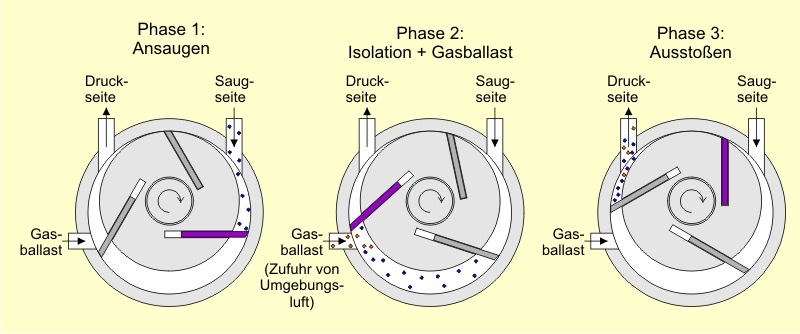
\includegraphics[width=\textwidth]{bilder/pumpe.jpeg}
    \caption{Schematischer Aufbau einer Drehschieberpumpe}
\end{figure}


\subsubsection{Turbomolekularpumpe}

Turbomolekularpumpen arbeiten effizient im Hochvakuumbereich und benötigen ein Vorvakuum, um effektiv zu funktionieren.
Dieses Vorvakuum wird durch eine vorgeschaltete Drehschieberpumpe erzeugt, die den Druck ausreichend senkt,
damit die Turbomolekularpumpe ihre Aufgabe erfüllen kann. Ohne diese Vorpumpe könnte die Turbomolekularpumpe nicht die erforderliche Geschwindigkeit erreichen,
um Gasmoleküle effektiv zu beschleunigen und ein hohes Vakuum zu erzeugen.
Die Turbomolekularpumpe ist eine mechanische Vakuumpumpe, die das Prinzip der molekularen Strömung nutzt.
Die Pumpe besteht aus einem Rotor und mehreren Statorscheiben. Der Rotor ist scheibenförmig und besitzt Schaufeln, die wie bei einer Turbine angeordnet sind.
Zwischen den Schaufeln befinden sich Spalten, die als Transportkanäle für das Gas dienen.
Durch den Ansaugstutzen wird das Gas in die Pumpe geleitet und gelangt dort in die Spalten zwischen den rotierenden Schaufeln. Durch die
hohe Geschwindigkeit des Rotors bekommen die Gasmoleküle Impulse übertragen, wodurch sie wiederholt mit den Schaufeln kollidieren können und so durch
die Pumpe transportiert werden. Die Moleküle werden in Richtung des Auslasses beschleunigt und bei erreichen des Auslassstutzen aus der Pumpe geleitet.
Dadurch wird der Druck in der Kammer verringert, was ein Vakuum erzeugt.
Die Pumpe basiert also auf der kinetischen Energie der Gasmoleküle. Die Pumpen sind besonders effektiv im Hochvakuumbereich
\cite{turbomolekularpumpe}.

\subsection{Vakuummessgeräte und Effizienzbereiche}
\subsubsection{Ionisations-Vakuummeter}
Die Ionisations-Vakuummeter sind in der Lage sehr niedrige Drücke präzise zu messen, sie werden also in Druckbereichen die dem Hochvakuum 
und dem Ultrahochvakuum entsprechen verwendet. In dem Gerät befindet sich ein Elektronenemitter, welcher Elektronen erzeugt. Diese
werden durch ein elektrisches Feld beschleunigt und ionisieren die Gasmoleküle sobald sie aufeinander treffen. Die entstandenen Ionen werden durch eine 
weiteres elektrisches Feld zu einer Sammel Elktrode hin beschleunigt. Dieser Ionenstrom ist proportional zu der Anzahl der ionisierten Moleküle im Vakuum und 
wird von einem Amperemeter gemessen. Da der Strom proportional zu der Gasdichte und damit zu dem Druck im Vakuum ist, kann der gemessene Strom einfach in einen 
Druckwert umgerechnet werden. Die Druckveränderungen entstehen also durch den Ionisationsprozess \cite{grundlagen_vakuumtechnik}.

\subsubsection{Glühkathoden und Kaltkathoden}

In einem Ionisationsvakummeter können sowohl Glühkathoden als auch Kaltkathoden verbaut werden. In der Praxis 
werden allerdings nicht beide Typen in einem Gerät vereint, sondern wählt nach Anforderungen an den Versuch welches
Gerät verwendet wird. Das Glühkathoden-Ionisationsvakuummeter arbeitet optimal im Hochvakuumbereich und nutzt die thermische
Emission von Elektronen durch das Erhitzen eines Glühdrahtes. Dieses Gerät kann sehr präzise Messungen durchführen und in niedrigen Druckbereichen arbeiten,
muss aber regelmäßig gewartet und gereinigt werden. Das Kaltkathode-Vakuummeter erzeugt Elektronenemission durch ein starkes elektrisches Feld.
Zusätzlich wird in der Kathode ein magnetisches Feld generiert, durch welches die Elektronen Schraubbewegungen durchführen und anschließend die
Ionisationen  erzeugen. Dieses Gerät ist weniger anfällig gegen Verschmutzungen und ist schneller einsetzbar als das Glühkathoden-Ionisationsvakummeter,
da es nicht erst eine bestimmte Betriebstemperatur erreichen muss, dafür ist es allerdings weniger präzise und kann im Hochvakuum nicht zuverlässig arbeiten
\cite{Kathoden}.


\subsubsection{Pirani-Vakuummeter}
Das Pirani-Vakuummeter ist ideal um mittlere Drücke im Bereich von $10^{-3}$ bar bis $10^{-2}$ bar zu messen.
Ein konstanter Strom erhitzt einen Draht aus Platin oder Wolfram, welcher sich in einem Gehäuse befindet, durch das Gas strömen kann.
Die Temperatur des Drahtes ist dabei abhängig von dem Druck des umgebenden Gases. Ist der Druck gering, so ist der Draht heiß.
Das liegt daran, dass das Gas bei wenig Druck und damit geringer Gasdichte ein schlechter Wärmeleiter ist und nur wenig Wärme vom 
Draht abführen kann. Mit der gleichen Argumentation ist der Draht bei hohem Druck kühler. Die Temperaturveränderung führt zu einer Veränderung
des elektrischen Widerstandes des Drahtes. Diese Veränderung wird mit einer Brückenschaltung gemessen und daraus kann dann der Druck bestimmt werden.
\cite{Vakuummeter}


\subsubsection{Piezo-Vakuummeter}
Das Piezo-Vakuummeter arbeitet effizient bei Druckbereichen von einem bar, also bei Atmosphärendruck.
In dem Vakuummeter befindet sich eine Membran, die von einem Gas umgeben ist. Der Druck des Gases übt eine Kraft auf die Membran aus,
wodurch diese sich verformt. Ist der Druck höher, so ist auch das Ausmaß der Verformung größer. Ein piezoelektrisches Material, welches sich direkt
an der Membran befindet kann die Verformung der Membran in ein elektrisches Signal übersetzen. Dieser Effekt wird piezoelektrischer Effekt bezeichnet, 
die Spannung entsteht durch die Verschiebung von elektrischen Ladungen innerhalb des Materials. Das Material muss dafür eine asymmetrische Kristallstruktur 
besitzen, sodass die positiven und negativen Ladungen im Kristall nicht symmetrisch verteilt sind. Der mechanische Druck auf das Material verschiebt die 
Atome innerhalb des Kristallgitters und damit die Verteilung der Ladungen im Material. Das daraus resultierende Dipolmoment erzeugt eine messbare elektrische
Spannung. Aus dieser Spannung kann der Druck bestimmt werden. Druck und Spannung sind proportional zueinander und zu der Verformung der Membran. 
\cite{Vakuummeter}